
\subsection{Temporal adaptation profile}

In summary, the results show that adaptation evidence in two different periods: 
1) in the earliest 2 hours of the embryo development ($\omega_{\alpha}$, $\omega_{d}$ and $\omega$ show their highest value at this stage) and 
2) from the L3 larval stage onwards, specially in the pupal and adult male stages which exhibit the highest levels of adaptive.

In between these stages of high adaptation, mid and late embryonic stages show high conservation. 
Similar results were found when considering after excluding immune system and testes genes (IV, Fig. S2) or when the mutation rate is estimated using the 4-fold degenerate sites (IV, Fig. S3).

The high adaptation rate in males is consistent with previous reports of higher adaptive substitutions in the genes expressed in males \citealp{Proschel2006,Haerty2007}). 
In contrast, based in a hybrid mis-expression assay with \textit{D. melanogaster} and \textit{D. sechellia}, \citet{Artieri2010} suggested a highly conserved pupal stage under strong stabilizing selection, which is contrary to the results shown in here, which indicate that, at least at the level of DNA coding sequence variation, pupal stages are among the least conserved.

As the morphology and other aspects of the phenotype of the larva and the adult arise primarily through the genetic, cellular and tissue interactions of embryonic and pupal development respectively, the adaptation in the larva or the adult morphology should be reflected in the genes expressed in embryonic development and pupal development, respectively.
Therefore, the evidence that most embryonic development shows low rates of adaptive change while the larva and pupa stages show higher rates of adaptative change suggests that there has been more adaptive changes in the adult morphology than in the larva morphology (between \textit{D. melanogaster} and \textit{D. yakuba}).

%%%%%%%%%%%%%%%%%%%%%%%%%%%%%%%%%%%%%%%%%%%%%%%%%%%%%%%
\begin{figure}[t]
  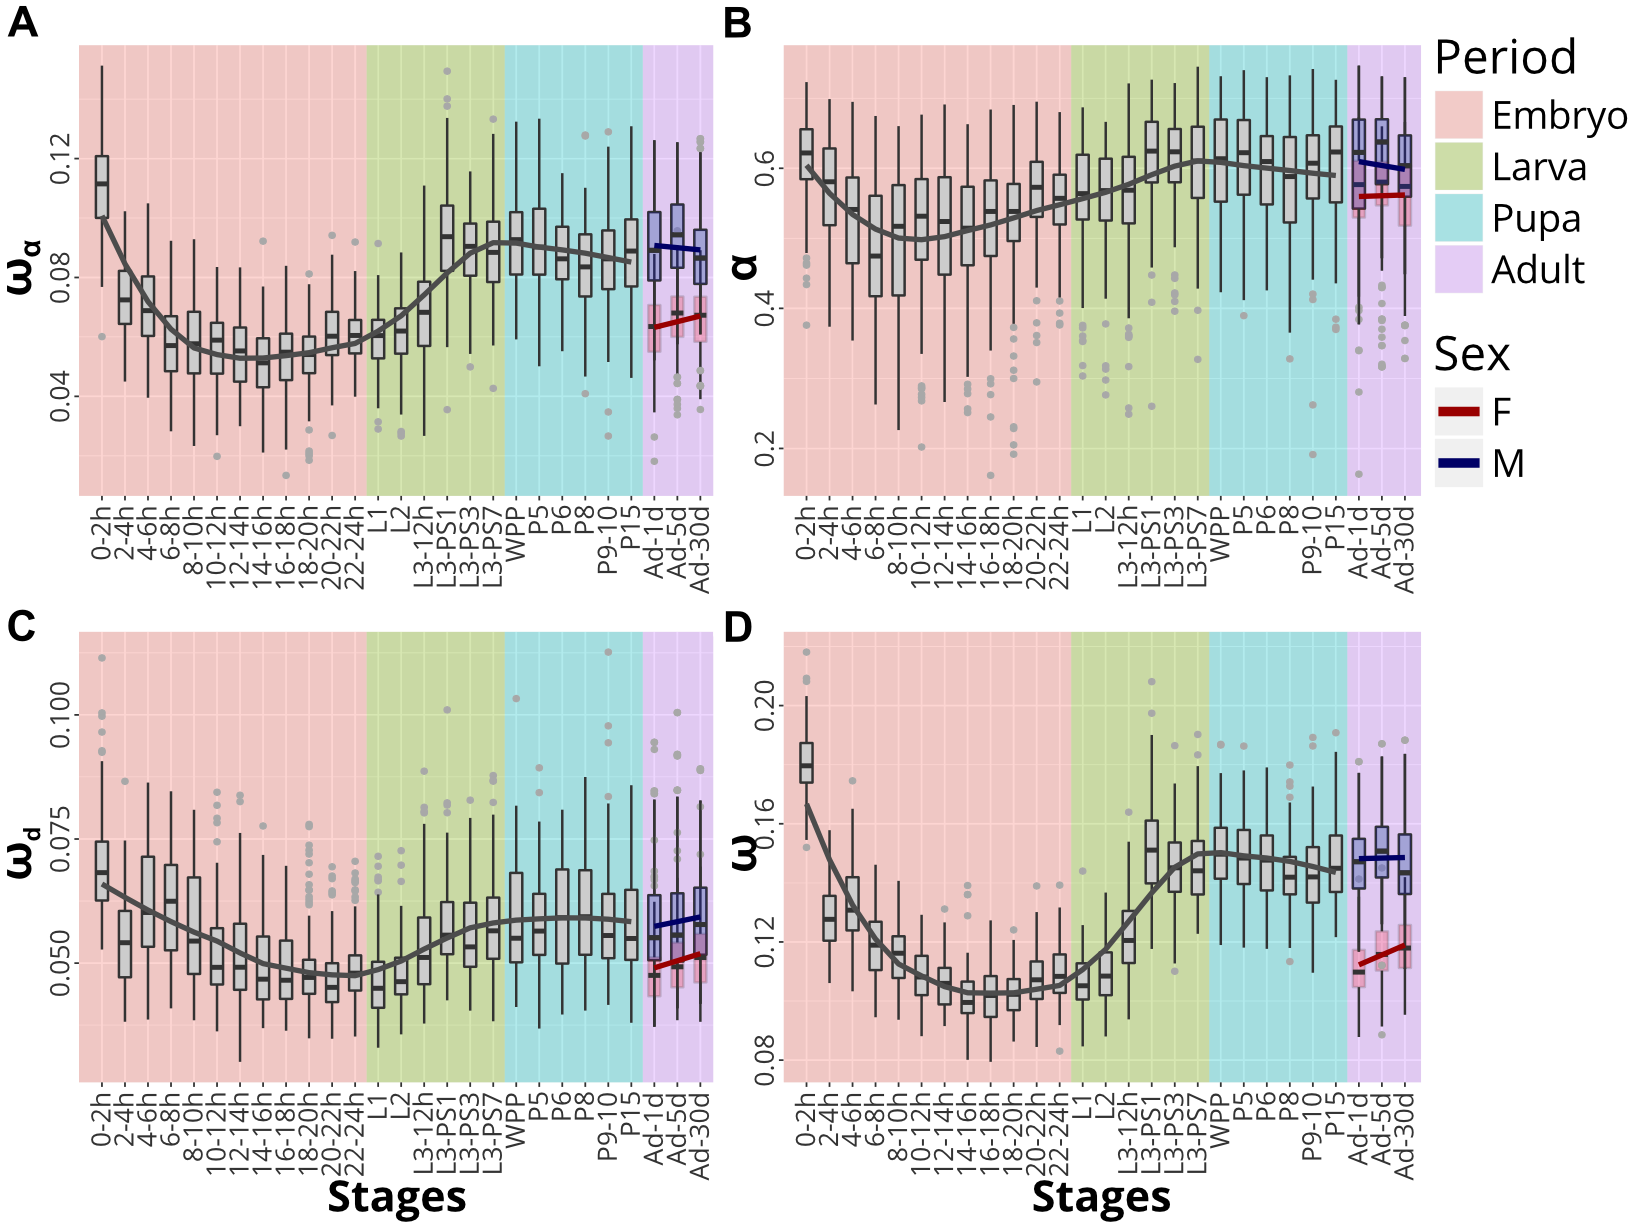
\includegraphics[width=\textwidth]{./Images/Art-IV/OmegaA_lifecycle.png}
  \centering
  \caption{\textbf{ {\large$\omega_{\alpha}$} (A),  {\large$\alpha$} (B), {\large$\omega_{d}$} (C), {\large$\omega$} (D) through the life cycle of \textit{D. melanogaster}} Each time point represents 1,000 random samples of 350 genes (with replacement) expressed in a stage. Red line represents a LOESS regression. Female and male stages are fitted to a linear regression. There are 12 embryonic stages at 2hr intervals (from 0h to 24h). Larval stages at first instar (L1), second instar (L2) and third instar (L3). L3 stages are subdivided into the first 12 hours (L3-12h) and several puff stage (L3-PS1 to L3-PS7). WPP is the white pre-pupae stage. Pupal stages are phanerocephalic pupa, 15h (P5), 25.6 hours pupa (P6), yellow pharate, 50.4 hours (P8), amber eye-pharate, 74.6 hours (P9-10), green meconium pharate, 96 hours (P15). Adult stages are 1, 5 and 30 days after eclosion (Ad-1d, Ad-5d, Ad-30d).
  }
  \label{fig:Art-IV-OmegaA_lifecycle}
\end{figure}
%%%%%%%%%%%%%%%%%%%%%%%%%%%%%%%%%%%%%%%%%%%%%%%%%%%%%%%%

\subsection{Results support the Hourglass model}

The temporal pattern of adaptation (and conservation) are roughly consistent with the Hourglass model (HG), specially for the early and mid embryonic development.
%This consistency is, however, rather weak since there are no major differences in ω between embryonic stages after the eight hour. 
During the first 6 hours $\omega$ and $\omega_{\alpha}$ are significantly high (permutation test), which is consistent with the expectations of the HG.
The same parameters are significantly lower during mid-embryogenesis, which is also consistent with the higher conservation expected from the HG, as the phylotypic stage (the most conserved stage) in \textit{Drosophila} has been suggested to be between the 6th and 10th hour \citep{Drost2015}.
However, during late embryonic stages (from 10-12h to 22-24h) $\omega$ and $\omega_{\alpha}$ are significantly lower (permutation test), which is not what is expected from the HG.

In contrast with some previous studies \citep{Davis2005,Kalinka2010} we do not find that the later stages of embryonic development are less conserved. 
It was found however, that a cluster composed of genes whose expression is high only in late development (done with a fuzzy clustering algorithm, cluster 8; see study IV), shows a significant $\omega$ and $\omega_{\alpha}$. In here, this group of genes have only a minor effect on the global pattern.
It could be that, due to the different methodology used by these other studies, these genes would have a relatively higher effect on the pattern observed. it could also be that the differences are partly due to the different species used in the analyses.\citet{Davis2005} use D. pseudoobscura as outgroup species while \citet{Kalinka2010} use six different \textit{Drosophila} species including \textit{D. melanogaster} but not \textit{D. yakuba}, the species used as outgroup in this work.

Despite these differences, the overall $\omega$ and $\omega_{\alpha}$ pattern (Fig \ref{fig:Art-IV-OmegaA_lifecycle}) is consistent with the HG model of embryonic development in \textit{Drosophila} \citep{Kalinka2010}.


%% result genomic determinants
\subsection{Correlation of adaptation with some genomic determinants}
Many "genomic determinants" temporal profiles correlate either positively other negatively with $\omega_{\alpha}$ (IV, Figs 2 and 3). 
%
Thus, messenger complexity (number of transcripts divided by the number of exons) correlates with $\omega_{\alpha}$ (rank correlation; see study IV). On the contrary, gene size, number of exons, codon usage bias and number of transcripts per gene negatively correlate with $\omega_{\alpha}$ (all with significant rank correlations; see study IV). 

This is consistent with previous studies that have shown that small gene size has been correlates with $\omega$ \citep{Duret1999,Comeron2012}.
%To our knowledge, the number of exons and transcripts themselves have never been directly associated with neither $\omega$ nor $\omega_{\alpha}$, as we found in our study.
It has also been suggested \citep{Gellon1998}, that developmental genes tend to have a complex gene structure with many exons and cis-regulatory elements and a complex regulation in space and time. Therefore, the correlations we observe between $\omega_{\alpha}$ and some genomic determinants is likely to simply reflect the fact that during mid-embryonic development, genes have a more complex spatio-temporal regulation and a more complex regulatory structure (as measure by the messenger complexity measure).

Based on the results shown in here, it is suggested that these genomic determinants can serve as predictors of adaptive change during development and that the temporal pattern of the genomic determinants are simply a consequence of the complex spatio-temporal regulation of gene expression occurring in embryonic 
development (as suggested on more qualitative grounds \citealp{Duboule1998}).

An important difference between this analysis and previous ones is that the DFE-alpha method allows to differentiate finely between conservation (indicated by low $\omega$), adaptive evolutionary substitution (high $\omega_{\alpha}$), non-adaptive substitution (high $\omega_{D}$) and the proportion of adaptive versus non-adaptive substitution (high $\alpha$). 
In a previous study, it was found that the 150 genes with the highest number of non-synonymous substitutions are expressed more strongly in larva and pupa than in embryo and that their highest level of expression is in male adults \citep{Davis2005}.
The work presented here would also be consistent with Davis et al., although in the latter case conservation and positive selection cannot be distinguished.


